\section{Methodology\label{sec:method}}

This section presents the methodology for studying how architectural signals and graph design choices affect code-to-architecture mapping. We formulate the mapping task as node classification over a software graph $G=(V, E,\mathcal{A},\mathcal{R})$, where $\mathcal{A}$ and $\mathcal{R}$ denote the sets of node and relation types. Let $V_f \subseteq V$ be the set of file nodes, which are the targets of the mapping task. A small subset $L \subset V_f$ is initially labeled with known architectural module assignments, and the remaining file nodes $U = V_f \setminus L$ are unlabeled. The objective is to learn an encoder:
\begin{equation}
Z = f_{\theta}(G), \qquad Z \in \mathbb{R}^{|V_f| \times d},
\end{equation}
that maps each source file $i\in V_f$ to a $d$-dimensional embedding $z_i$, where $\theta$ denotes the learnable parameters of the representation-learning method. These file embeddings are used to predict architectural modules and to infer the labels of the nodes in $U$.
 
We first describe the graphs and the structural, lexical, and contextual features used to initialize their nodes. We then present the graph-free MLP, the HGT encoder, and their iterative training procedure. RQ1 varies the file representation, using the graph-free MLP. RQ2 varies the graph configuration for each representation and compares the results with a directory baseline described in Section~\ref{sec:dir_predictor}. RQ3 fixes the representations and varies neighbor information, predictor, and training schedule, as described in Section~\ref{sec:controlled_setup}.

 % _______ Graph Construction ___________
\subsection{Heterogeneous Graph Construction\label{sec:het_graph}}
We model the software system as a heterogeneous graph whose nodes represent software artifacts and edges represent organizational, containment, and dependency relations. The graph is built from three sources of information: the folder structure of the project, the containment of program elements within a file, and static dependencies extracted from source code. Folder structure provides organizational context, containment connects folders to the files they contain and members to the files they belong to, and static dependencies describe interactions between software entities. We preserve these sources as distinct node and relation types rather than collapsing them into a single homogeneous graph. Figure~\ref{fig:schema} illustrates the general schema of the heterogeneous software graph and the meta-relations used in our model.
 
\begin{figure}[!h]
\centering
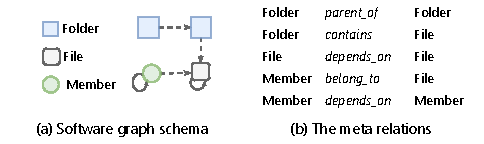
\includegraphics[width=1\linewidth]{Images/hetmap_schema.pdf}
\caption{Schema and meta-relations of the heterogeneous software graph. The figure shows the most expressive representation, with folder, file, and member nodes. Simpler variants remove selected node types or aggregate member-level dependencies at the file level.\label{fig:schema}}
\end{figure}
 
\subsubsection{Node Types}
We use three node types: folder, file, and member. Folder nodes represent directory levels in the project structure. File nodes represent source files and are the target nodes for code-to-architecture mapping. Member nodes represent member-level program information associated with a file, including methods, fields, constructors, and variables.
 
We use one summarized \textit{Member} node per file rather than representing each method, field, constructor, or variable as a separate node. The member node aggregates lexical and dependency information from the members of its associated file, retaining member-level information while avoiding the large and sparse graphs produced by fully fine-grained representations.

\subsubsection{Relation Types}
The graph contains structural relations, including organization, containment, and dependency. Logical components are often implemented through namespaces or directory structures that group source code providing a particular functionality, and such structures reflect how developers organize files~\cite{fundamentals_sa, garcia2013}. To preserve this information, each directory level is represented as a separate folder node. Folder nodes are connected through \emph{parent\_of} edges, forming hierarchical chains such as \texttt{app} $\rightarrow$ \texttt{app/ui} $\rightarrow$ \texttt{app/ui/views}. File nodes are linked to their folder through \emph{contains} edges, and each member node is connected to its enclosing file through a \emph{belongs\_to} edge.

Static dependencies provide direct evidence of how entities interact and are a central source of information for architecture mapping and recovery~\cite{negar, deps_impact}. The frozen dependency artifacts were extracted with the Depends tool~\cite{depends}, which analyzes the syntactic structure of the projects studied in this paper and identifies entities together with several categories of static relations. Different dependency types can carry distinct architectural meanings~\cite {edge_weights, sarif}, so we keep them as separate relational edge types rather than merging them into a single dependency relation. Table~\ref{tab:relation_types} lists the structural relations introduced during graph construction and the static dependency types observed in the analyzed Java and C/C++ systems.

\begin{table}[htb]
\centering
\caption{Structural and static dependency relation types used in the software graph.}
\label{tab:relation_types}

\renewcommand{\arraystretch}{1}
\begin{adjustbox}{max width=\columnwidth}
\begin{threeparttable}
\begin{adjustbox}{max width=\columnwidth}
\begin{tabular}{ll}
\toprule
\textbf{Relation type} & \textbf{Description} \\
\midrule
\emph{parent\_of} & Folder contains a subfolder in the directory. \\
\emph{contains} & Folder contains a source file. \\
\emph{belongs\_to} & Member-level program element belongs to a file. \\
\midrule
\texttt{Call} & Function or method invocation. \\
\texttt{Cast} & Conversion of an entity to another type. \\
\texttt{Contain} & Definition or containment of variables/fields. \\
\texttt{Create} & Creation of an instance or program entity. \\
\texttt{Extend} & Inheritance or parent-child type relation. \\
\texttt{Implement} & A class implements an interface or abstraction. \\
\texttt{Import} & A file imports other classes, methods, or variables. \\
\texttt{Parameter} & Use of a type as a method or function parameter. \\
\texttt{Return} & Use of a type as a return type. \\
\texttt{Use} & Use or assignment of variables. \\
\bottomrule
\end{tabular}
\end{adjustbox}
\begin{tablenotes}[flushleft]
\item \texttt{Annotation} and \texttt{Throw} are not observed in the C/C++ systems.
\end{tablenotes}
\end{threeparttable}
\end{adjustbox}
\end{table}

\subsubsection{Graph Variants\label{sec:graph_variants}}
Folder organization, member-level information, and static dependencies are available simultaneously in the complete graph, so their contributions cannot be determined from the full configuration alone. We therefore construct four graph variants that vary the presence of folder and member nodes while retaining dependency information at the available granularity. Figure~\ref{fig:graph_variants_overview} provides a visual overview; Table~\ref{tab:graph_variants} summarizes their roles. Files are always the prediction targets. A member node summarizes a file's program members, while folder nodes supply directory context.

\begin{figure}[tb]
\centering
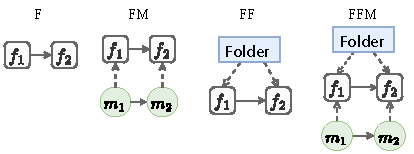
\includegraphics[width=1\linewidth]{Images/graph_variants.pdf}
\caption{Graph configurations: files $f_i$ are the prediction targets; each $m_i$ aggregates the members of file $f_i$. Solid arrows show dependencies and dashed arrows show meta-relations. The panels omit relation types, additional dependency edges, and folder ancestry; Figure~\ref{fig:schema} gives the typed schema. Feature construction also depends on the configuration, as described in Section~\ref{sec:node_features}.\label{fig:graph_variants_overview}}
\end{figure}

We classify dependencies according to their resolved endpoints. A dependency is file-level if at least one endpoint is a file; this includes file--file, file--member and member--file interactions. It is member-level if both endpoints are members. FFM keeps these dependency edges separate from containment relations and preserves their endpoint types. FM removes folder nodes and relations while retaining files and members. FF and F also remove member nodes. In these variants, each member endpoint is replaced by its enclosing file, so all remaining dependencies connect file nodes.

\begin{table}[!ht]
\centering
\caption{Graph variants used to study the effect of graph granularity and information sources.}
\label{tab:graph_variants}
\begin{adjustbox}{max width=\columnwidth}
\Large
\begin{tabular}{l l l}
\toprule
\textbf{Variant} & \textbf{Node types} & \textbf{Purpose} \\
\midrule
FFM & Folder, File, Member & Complete heterogeneous structure \\
FF & Folder, File & Folder and file-level structure \\
FM & File, Member & Member-level structure without folders \\
F & File & File-level dependency baseline \\
\bottomrule
\end{tabular}
\end{adjustbox}
\end{table}
% _________ Node Feature Initialization ______________

\subsubsection{Relation Types}
The graph contains structural relations, including organization, containment, and dependency. Logical components are often implemented through namespaces or directory structures that group source code providing a particular functionality, and such structures reflect how developers organize files~\cite{fundamentals_sa, garcia2013}. To preserve this information, each directory level is represented as a separate folder node. Folder nodes are connected through \emph{parent\_of} edges, forming hierarchical chains such as \texttt{app} $\rightarrow$ \texttt{app/ui} $\rightarrow$ \texttt{app/ui/views}. File nodes are linked to their folder through \emph{contains} edges, and each member node is connected to its enclosing file through a \emph{belongs\_to} edge.
 
Static dependencies provide direct evidence of how entities interact and are a central source of information for architecture mapping and recovery~\cite{negar, deps_impact}. Dependencies were extracted with the Depends tool~\cite{depends}, which analyzes the syntactic structure of the projects studied in this paper and identifies entities together with several categories of static relations. Different dependency types can carry distinct architectural meanings~\cite{edge_weights, sarif}, so we keep them as separate relational edge types rather than merging them into a single dependency relation. Table~\ref{tab:relation_types} lists the structural relations introduced during graph construction and the static dependency types observed in the analyzed Java and C/C++ systems.
 
\begin{table}[htb]
\centering
\caption{Structural and static dependency relation types used in the software graph.}
\label{tab:relation_types}
 
\renewcommand{\arraystretch}{1}
\begin{adjustbox}{max width=\columnwidth}
\begin{threeparttable}
\begin{adjustbox}{max width=\columnwidth}
\begin{tabular}{ll}
\toprule
\textbf{Relation type} & \textbf{Description} \\
\midrule
\emph{parent\_of} & Folder contains a subfolder in the directory. \\
\emph{contains} & Folder contains a source file. \\
\emph{belongs\_to} & Member-level program element belongs to a file. \\
\midrule
\texttt{Call} & Function or method invocation. \\
\texttt{Cast} & Conversion of an entity to another type. \\
\texttt{Contain} & Definition or containment of variables/fields. \\
\texttt{Create} & Creation of an instance or program entity. \\
\texttt{Extend} & Inheritance or parent-child type relation. \\
\texttt{Implement} & A class implements an interface or abstraction. \\
\texttt{Import} & A file imports other classes, methods, or variables. \\
\texttt{Parameter} & Use of a type as a method or function parameter. \\
\texttt{Return} & Use of a type as a return type. \\
\texttt{Use} & Use or assignment of variables. \\
\bottomrule
\end{tabular}
\end{adjustbox}
\begin{tablenotes}[flushleft]
\item \texttt{Annotation} and \texttt{Throw} are not observed in the C/C++ systems.
\end{tablenotes}
\end{threeparttable}
\end{adjustbox}
\end{table}
 
\subsubsection{Graph Variants\label{sec:graph_variants}}
Folder organization, member-level information, and static dependencies are available simultaneously in the complete graph, so their contributions cannot be determined from the full configuration alone. We therefore construct four graph variants that vary the presence of folder and member nodes while retaining dependency information at the available granularity. Figure~\ref{fig:graph_variants_overview} provides a visual overview. Files are always the prediction targets, a member node summarizes a file's program members, and folder nodes supply directory context.
 
\begin{figure}[tb]
\centering
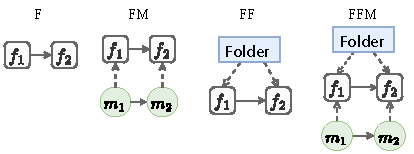
\includegraphics[width=1\linewidth]{Images/graph_variants.pdf}
\caption{\small Graph configurations: files $f_i$ are the prediction targets; each $m_i$ aggregates the members of file $f_i$. Solid arrows show dependencies and dashed arrows show meta-relations. The panels omit relation types, additional dependency edges, and folder ancestry; Figure~\ref{fig:schema} gives the typed schema. Feature construction also depends on the configuration, as described in Section~\ref{sec:node_features}.\label{fig:graph_variants_overview}}
\end{figure}
 
We classify dependencies according to their resolved endpoints. A dependency is file-level if at least one endpoint is a file; this includes file--file, file--member, and member--file interactions. It is member-level if both endpoints are members. FFM is the complete graph and keeps these dependency edges separate from containment relations, preserving their endpoint types. FM removes folder nodes and relations while retaining files and members. FF removes member nodes instead, and F removes both folder and member nodes and serves as the file-level dependency baseline. In FF and F, each member endpoint is replaced by its enclosing file, so all remaining dependencies connect file nodes. The controlled experiments also use a homogeneous version of F, in which dependency direction and edge types are removed.
 
% _________ Node Feature Initialization ______________
\subsection{Node Feature Initialization \label{sec:node_features}}
We initialize node features based on the information source used in each experimental setting. Folder nodes are always initialized from binary folder-path tokens, regardless of which strategy is used elsewhere in the graph. File and member nodes are initialized using one of three strategies: lexical embeddings from Word2Vec, structural embeddings from Node2Vec, or contextual embeddings from UniXcoder, used zero-shot or fine-tuned with dependencies as described below.
 
\subsubsection{Folder Node Features}
 
Folder nodes are encoded using a binary bag-of-words representation over folder tokens. The folder tokens are derived from directory segments after removing common project-root tokens. Each folder node is represented by the tokens along its path in the directory hierarchy. For example, a folder corresponding to \texttt{app/ui/views} carries the tokens \texttt{app}, \texttt{ui}, and \texttt{views}. This allows deeper folder nodes to retain information about their hierarchical context.
 
\subsubsection{Word2Vec: Lexical Features \label{sec:node_w2v}}
Source code identifiers often encode domain concepts and implementation roles, making them useful cues for mapping entities to architectural modules~\cite{sarif}. We use Word2Vec embeddings following the approach of Jabeen et al.~\citep{gaer} for lexical input. Tokens are extracted from file names and member-level program elements, including methods, fields, constructors, and variables. We normalize identifiers by splitting camelCase, PascalCase, and snake\_case forms, converting tokens to lowercase, and removing stopwords and non-alphabetic tokens. The remaining tokens are represented using 128-dimensional skip-gram Word2Vec embeddings~\cite{word2vec}, trained for 20 epochs with a context window of five. Each node representation is computed by averaging the embeddings of its associated tokens.
 
The graph variant determines where these features are stored. In FFM and FM, the file node contains file-name tokens and the member node contains identifiers from the file's program elements. FF and F have no member nodes, so member identifiers are included in the file representation instead, and the graph-free MLP uses the same file vector as F and FF. Member identifiers therefore remain available in every variant, but moving to FM or FFM changes where the information enters the model as well as changing the graph and its parameters.
 
\subsubsection{Node2Vec: Structural Features \label{sec:node_n2v}}
Chen et al.~\citep{negar} observe that files in the same architectural module can occupy a dense local dependency region without being directly connected. Shallow message passing over raw dependency graphs can therefore provide too limited a context to expose such relationships, whereas random walks can capture longer-range dependency structure~\cite{structsar}. We use Node2Vec's~\cite{node2vec} random-walk embeddings as a structural initialization and merge all static dependency types into a single edge type before generating random walks. Its biased random walks use parameters $p$ and $q$ to balance local and exploratory walks. The resulting embeddings capture structural similarity from dependency position without using identifier text or folder location.
 
In FM and FFM, each aggregate member node receives the Node2Vec embedding of its corresponding file. These configurations therefore change graph processing without introducing a separately learned member-level structural embedding.
 
\subsubsection{UniXcoder: Contextual Features \label{sec:unixcoder}}
For contextual initialization, we use UniXcoder~\cite{unixcoder}, a pretrained code transformer. The zero-shot variant uses its pretrained weights directly. The dependency-guided variant fine-tunes the encoder separately for each system using that system's dependency structure.
 
Source files are parsed with tree-sitter~\cite{tree_sitter} to produce separate file and member views. For Java, the file view contains type headers, field declarations, and constructor signatures with short body excerpts. The member view contains ordinary method declarations and excludes constructors. C/C++ extraction uses the appropriate language grammars to separate type and state declarations, including applicable constructors, from ordinary operations. It preserves physical-file boundaries and does not expand includes or macros. Unlike Word2Vec, UniXcoder does not move the member text into the file view when member nodes are absent.
 
Jabeen et al.~\cite{structsar} show that shallow message passing over the raw dependency graph struggles to expose relationships between files that are connected only through shared neighbors rather than a direct edge. Therefore, positive pairs for contrastive fine-tuning are drawn primarily from the two-hop neighborhood: for each anchor file, two-hop candidates are ranked by the number of distinct one-hop neighbors shared with the anchor, and two pairs per file are sampled from the top eight candidates; files without any two-hop candidates fall back to a direct neighbor. Training uses an InfoNCE~\cite{infonce} objective with in-batch negatives; in-batch items connected by dependencies but not selected as a positive pair are masked so that they act as neither positive nor negative.
 
Only the upper four encoder layers are updated during fine-tuning, while the token embedding layer and the lower eight encoder layers stay frozen, since the number of dependency pairs available in a single system is small relative to the encoder's parameter count. Adaptation is performed independently for each subject system, as dependency structure and naming conventions are project-specific.
 
Member information therefore enters the model differently for each representation. W2V moves member identifiers from the file vector to the member node when member nodes are present, UniXcoder provides member text only through the member node, and N2V gives the member node the file's own vector. Moving from F to FM or FFM thus changes how information enters the model as well as the graph, and the comparisons across graph variants are interpreted for each representation separately.
% __________ Model ________________
\subsection{Mapping Models\label{sec:mapping_models}}
All models map the final file representation to module logits with a linear layer and are trained by minimizing categorical cross-entropy over the labeled file nodes. They differ in how that file representation is computed.

\subsubsection{Multilayer Perceptron (MLP)\label{sec:mlp}}
The MLP predicts module logits directly from a file-level input vector. Each hidden layer computes:
\begin{equation}
h_i^{(k+1)} = \text{ReLU}\big(W^{(k)} h_i^{(k)} + b^{(k)}\big),
\end{equation}
with $h_i^{(0)} = x_i$ the file feature vector and $W^{(k)}, b^{(k)}$ the learnable parameters of layer $k$, and ReLU is the rectified linear unit~\cite{relu}. After the final hidden layer, a linear layer maps the resulting representation to module logits. The input $x_i$ contains the single representation being evaluated.

\subsubsection{Heterogeneous Graph Transformer (HGT)\label{sec:hgt_model}}
Node types have different feature spaces depending on the graph variant and the initialization strategy, so the HGT-based model first maps each node type into a shared hidden space using a type-specific linear transformation followed by ReLU. One HGT layer~\cite{hgt} then updates node representations through multi-head attention over their neighbors. Attention uses target-type-specific query transformations, source-type-specific key transformations, edge-type-specific matrices, and a learned prior for each meta-relation. Messages use source-type-specific transformations and edge-type-specific matrices. These parameters allow a \emph{contains} edge from a folder and a \texttt{Call} edge from a dependent file to receive different attention weights. In our implementation, the aggregated messages are combined with the node's projected input through a residual connection followed by layer normalization:
\begin{equation}
h_t^{(1)} = \mathrm{LayerNorm}\left(\sum_{s \in \mathcal{N}(t)} \alpha(s,e,t) \cdot M(s,e,t) + h_t^{(0)}\right),
\end{equation}
where $\alpha(s,e,t)$ and $M(s,e,t)$ denote the attention weight and message from source node $s$ to target node $t$ over edge $e$, with attention-head indices omitted for brevity, and $h_t^{(0)}$ is the projected input. The residual connection retains a direct path from the initial node features~\cite{residual_connection}. Folder and member nodes, when present, contribute to file representations through message passing.

\subsubsection{Graph Attention Network (GAT)\label{sec:gat_model}}
GAT~\cite{gat} aggregates neighbor representations with a single attention mechanism shared by all neighbors, without the node-type-, edge-type-, or direction-specific parameters of HGT. Like HGT, it first projects the input vector and combines the aggregated messages with the projected input through a residual connection followed by layer normalization:
\begin{equation}
h_i^{(1)} = \mathrm{LayerNorm}\left(\Big\Vert_{k=1}^{K} \sum_{j \in \mathcal{N}(i)} \alpha_{ij}^{(k)} W^{(k)} h_j^{(0)} + h_i^{(0)}\right),
\end{equation}
where $\Vert$ denotes concatenation over the $K$ attention heads, $\alpha_{ij}^{(k)}$ is the attention weight of neighbor $j$ for node $i$ in head $k$, $W^{(k)}$ is a head-specific learnable matrix, and $h_i^{(0)}$ is the projected input.

% ________ Algorithm _____________
\subsection{Iterative Learning Framework\label{sec:iterative_learning}}
The configuration experiments use a common form of iterative self-training: predictions above a confidence threshold supplement the initial labels. The thresholds and maximum round counts differ across models, as detailed in Section~\ref{sec:exp_setup}. The controlled experiments additionally fix the training duration and include a supervised-only schedule.

Starting from the labeled set $L$, the model first trains in a supervised warm-up phase on $L$. It then scores every file node with a softmax over the predicted modules; the highest probability is the model's confidence in that prediction. In each self-training round, unlabeled file nodes whose confidence exceeds a threshold $\delta$ receive pseudo-labels and are added to $L_{\text{pseudo}}$, and the model is retrained on the union of the original and pseudo-labeled nodes. If a later round predicts a different label for a pseudo-labeled node with confidence above $\delta$, the pseudo-label is updated. The procedure stops when no new confident nodes are found, when fewer than five nodes were added in the previous round, or when the maximum number of self-training rounds is reached. The fixed-budget self-training schedule of the controlled experiments in RQ3 disables these early stopping conditions and completes all three rounds, including rounds with no new pseudo-labels.

% \begin{algorithm}
% \footnotesize
% \caption{Adaptive self-training for the configuration experiments.\label{alg:iter_hetmap}}
% \KwIn{Input representation $\mathcal{I}$, file nodes $\mathcal{F}$, labeled set $L$, confidence threshold $\delta$, warm-up epochs $E_w$, self-training epochs $E_s$, max rounds $R$}
% \KwOut{Trained classifier $f$, pseudo-labeled set $L_{\text{pseudo}}$}
% $L_{\text{pseudo}} \gets \emptyset$;\ $U \gets \mathcal{F} \setminus L$\;
% Train $f$ on $(\mathcal{I}, L)$ for $E_w$ epochs\;
% $\text{added} \gets \infty$\;
% \For{$k \gets 1$ \KwTo $R$}{
%     \If{$\text{added} < 5$}{\textbf{break}\;}
%     Score all files in $\mathcal{F}$ with $f$ using $\mathcal{I}$\;
%     Revise any pseudo-label in $L_{\text{pseudo}}$ whose confidence $> \delta$ disagrees with $f$\;
%     $\mathcal{P} \gets \{o \in U \mid \text{confidence}(o) > \delta\}$\;
%     \If{$\mathcal{P} = \emptyset$}{\textbf{break}\;}
%     $\text{added} \gets |\mathcal{P}|$\;
%     $L_{\text{pseudo}} \gets L_{\text{pseudo}} \cup \mathcal{P}$;\ $U \gets U \setminus \mathcal{P}$\;
%     Retrain $f$ on $(\mathcal{I}, L \cup L_{\text{pseudo}})$ for $E_s$ epochs\;
% }
% \Return{$f$, $L_{\text{pseudo}}$}\;
% \end{algorithm}

